\section{Installing and Starting}

\subsection{Desktop Application}

The desktop application requires the Java Runtime Environment (JRE) available
from \url{http://www.java.com/en/download/index.jsp}. The application has been
tested on JRE 6 and JRE 7 without issue. The print functionality
requires a pre-installed \LaTeX distribution that includes the
executable `pdflatex'. The installation procedure varies for each
operating system and instructions are available from:
\url{http://latex-project.org/ftp.html}.

After the Java Runtime Environment (JRE) is installed, running the application
can be achieved by executing the following command from any terminal
window:
\begin{verbatim}
java -jar TeamW-SportsElim.jar
\end{verbatim}
or by launching from your favourite file browser.

A \LaTeX  distribution is not required to run the core of the
application, only the print functionality. In the event that the
command `pdflatex' cannot be found, the application will fail to print
however will not crash. Print functionality is known to work on
standard installations of the distribution on Linux/GNU-based and Mac
OS operating system.

\subsection{Web Application}
\label{sec:WEBAPP}
Installation of the web application is not required as a remote host is running
the required software. This can be accessed via
\url{http://www.gordonrenfrewshire.com/teamw}. For purposes of completeness and
satisfying the potential desires of the reader, an installation procedure was
supplied in Appendix~\ref{sec:install}.

In the event that the supplied URL fails to work, please contact Gordon Reid via
any of the following methods:

Student email: 1002536r@student.gla.ac.uk

Personal email: gordon.reid1992@hotmail.co.uk

Mobile phone: 07706 477 672

\section{Desktop Navigation}

\begin{figure}
  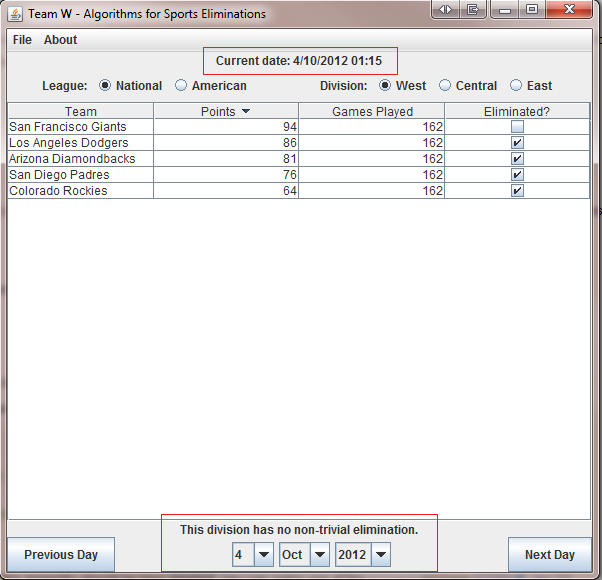
\includegraphics[width=\linewidth,keepaspectratio]{images/userManualDesk1.png}
  \caption{Starting Screen}\label{fig:STARTSCREEN}
\end{figure}
Upon launching, you will see the screen in Figure~\ref{fig:STARTSCREEN}.
Highlighted in the red box at the bottom of the screen is the
main navigational tool for traversing to different dates within the
season. Three drop-down selectors allow you to instantly jump to any
date in the season. Simple day-by-day navigation can be achieved
using the buttons in the bottom left and bottom right of
Figure~\ref{fig:STARTSCREEN} and these allow you to navigate backwards
or forwards in the league respectively.
The application will always start at the last date in the season it
knows about. The current date and time relating to the information on
screen is displayed in the red box at the top of the screen.

\begin{figure}
  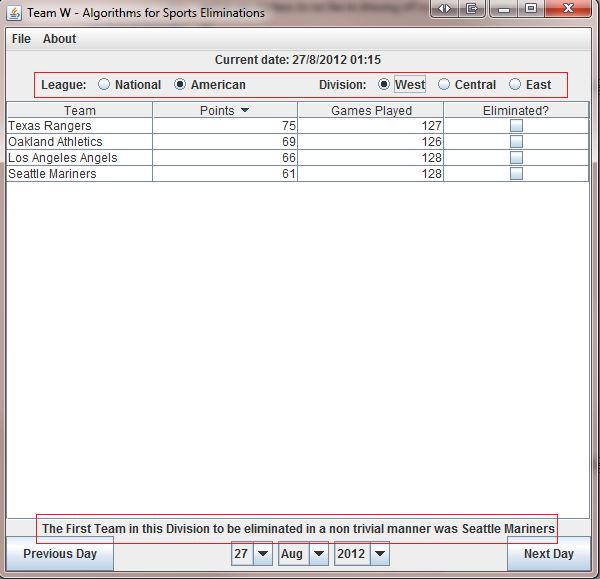
\includegraphics[width=\linewidth,keepaspectratio]{images/userManualDesk3.png}
  \caption{League Navigation}\label{fig:LEAGNAV}
\end{figure}
The radio buttons highlighted at the top of Figure~\ref{fig:LEAGNAV}
allow you to change between the various divisions supported by the
application. There are a total of six combinations. The date you
are currently on transfers when you change league, for example if you
are viewing the ``National West'' division on ``27/8/2012 01:15'' and
you change to ``National East'' you will see the results of the
``National East'' division on ``27/8/2012 01:15''. The first
non-trivial elimination information for the currently selected
division is shown in the highlighted red box at the bottom of
Figure~\ref{fig:LEAGNAV}.

\begin{figure}
  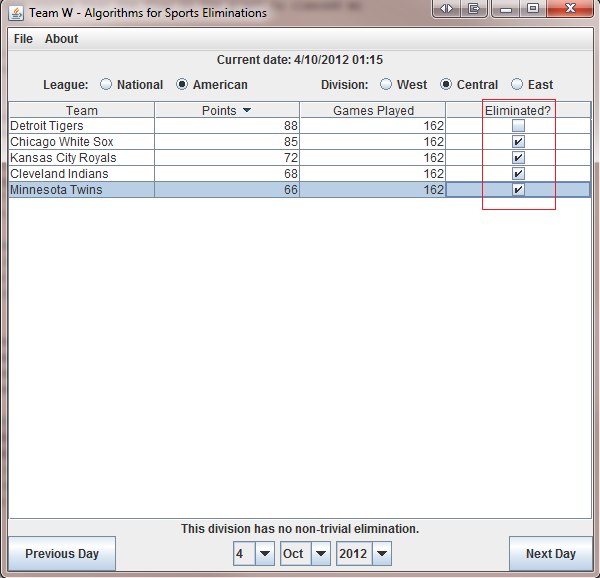
\includegraphics[width=\linewidth,keepaspectratio]{images/userManualDesk4.png}
  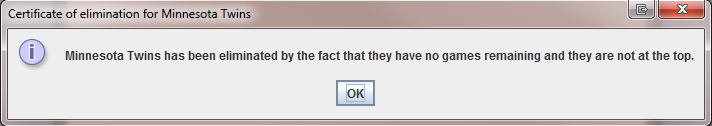
\includegraphics[width=\linewidth,keepaspectratio]{images/userManualDesk5.png}
  \caption{Elimination Status}\label{fig:ELIMSTAT}
\end{figure}

Figure~\ref{fig:ELIMSTAT} demonstrates viewing the reason for why a
specific team has been eliminated. Highlighted in red, the
``Eliminated?'' check-boxes are ticked if a team has been eliminated
on the current date. Clicking on a ticked check-box will display the
popup giving the reason for the selected teams elimination. The pop-up
will only show if a team has been eliminated.

\newpage

\section{Importing}
\label{sec:Importing}
The import functionality within the application allows user specified
seasons to be used in the system directly. If analysis of future or
prior seasons is desired then these can be imported into the
application with ease by selecting ``File$\rightarrow$Open...'' and importing a
correctly formatted file. A user is also permitted to import their own
custom league provided that the correct format is used and the
required teams exist within the file. When the file has been imported,
the application will show you the latest results found inside the file
and will allow you the normal navigation.

\section{Generation of Leagues}
As shown in Figure~\ref{fig:GENPIC}, generating a league can be
achieved in a simple manner. Following the commands highlighted in the
red boxes will bring up a dialogue box asking for a destination file
to save the generated league in and then you will be informed of the
generations success. This generated league can be manipulated at will
and imported by following the instructions in~\ref{sec:Importing}
\begin{figure}
  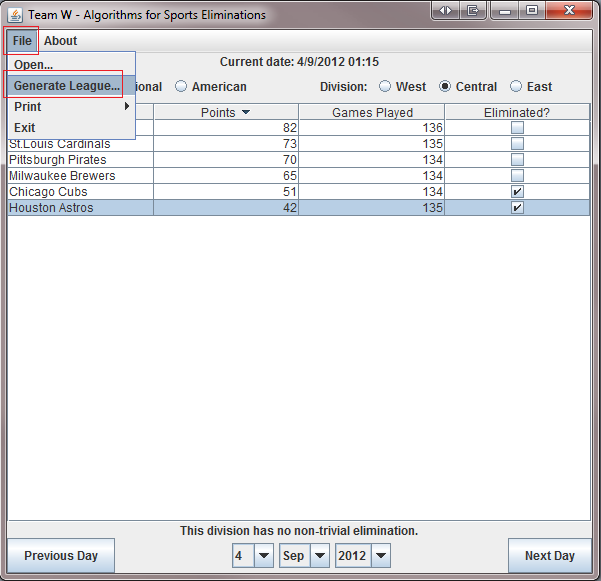
\includegraphics[width=\linewidth,keepaspectratio]{images/userManualDesk7.png}
  \caption{Generation of a random league}\label{fig:GENPIC}
\end{figure}

\section{Exporting}

The export functionality allows users to create a PDF file with
selected information. Following the commands highlighted in
Figure~\ref{fig:EXPORT} allows you to add the division information as
it appears on screen to the document.

\begin{figure}
  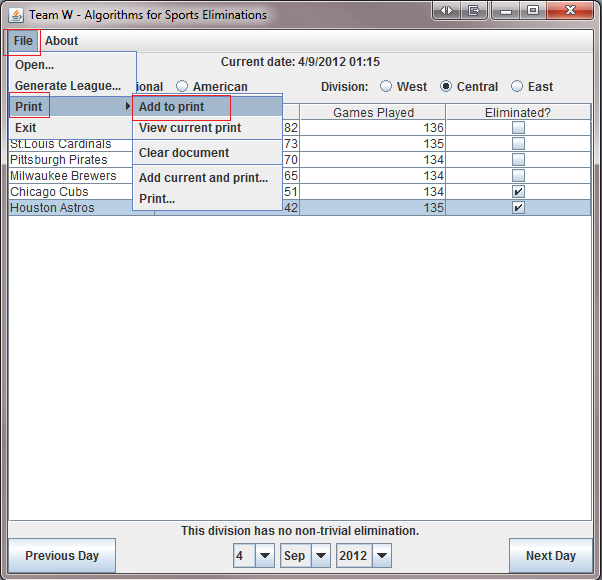
\includegraphics[width=\linewidth,keepaspectratio]{images/userManualDesk9.png}
  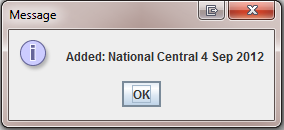
\includegraphics{images/userManualDesk10.png}
  \caption{Export Functionality}\label{fig:EXPORT}
\end{figure}


At any time you can follow the steps in Figure~\ref{fig:EXPVIEW} to
see the information that is ready to be exported.

\begin{figure}
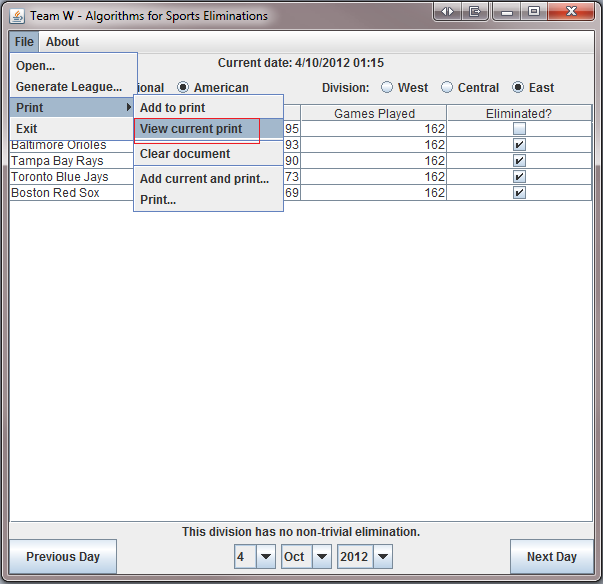
\includegraphics[width=\linewidth,height=\measurepage,keepaspectratio]{images/userManualDesk11.png}
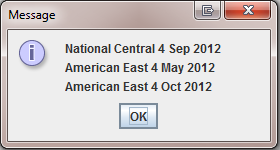
\includegraphics{images/userManualDesk12.png}
\caption{Viewing information to be exported}\label{fig:EXPVIEW}
\end{figure}

Finally you can either clear your print queue by selecting ``Clear document'', or
to export your selected results to the PDF select ``Print''. The
option between the two highlighted boxes in Figure~\ref{fig:EXPEXP}
allows the user to export the current league at the current date
instantly. A prompt will ask you to select a name for your PDF file in a dialogue box and a
location to save it and then by clicking save your PDF will be compiled ready
for viewing at the specified location.

\begin{figure}
  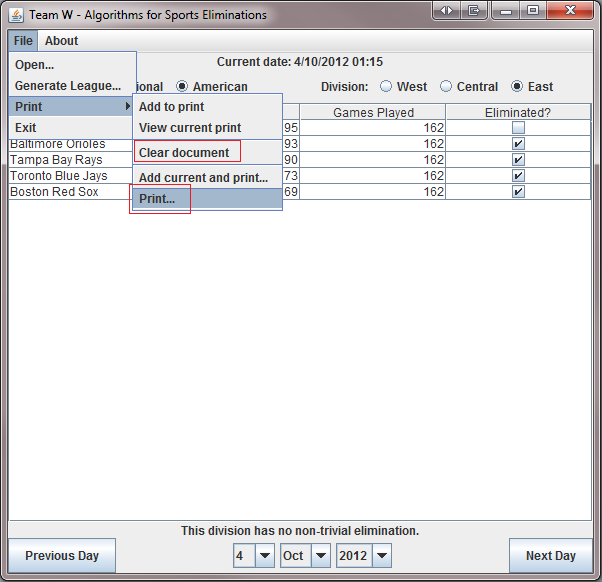
\includegraphics[width=\linewidth,keepaspectratio]{images/userManualDesk13.png}
  \caption{Exporting}\label{fig:EXPEXP}
\end{figure}
\newpage

\section{Web Navigation}

Upon navigating to the URL specified in the installation
chapter~\ref{sec:WEBAPP} you will be shown this screen in Figure~\ref{fig:WEBHOME}.

\begin{figure}
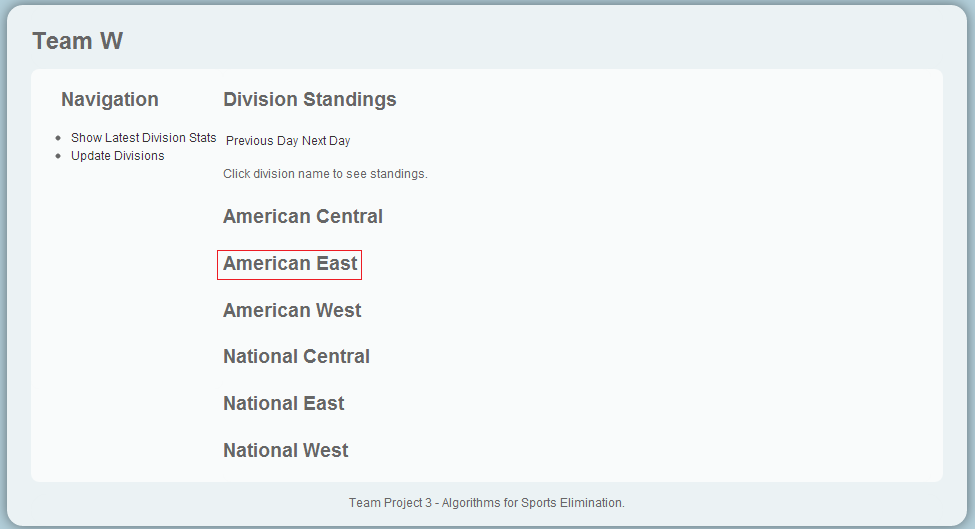
\includegraphics[width=\linewidth,keepaspectratio]{images/userManualWeb1.png}
\caption{Web Application Landing Screen}\label{fig:WEBHOME}
\end{figure}

If you click on any of the emboldened division headings the standings will be
displayed below as shown in Figure~\ref{fig:WEBINFO}.

\begin{figure}
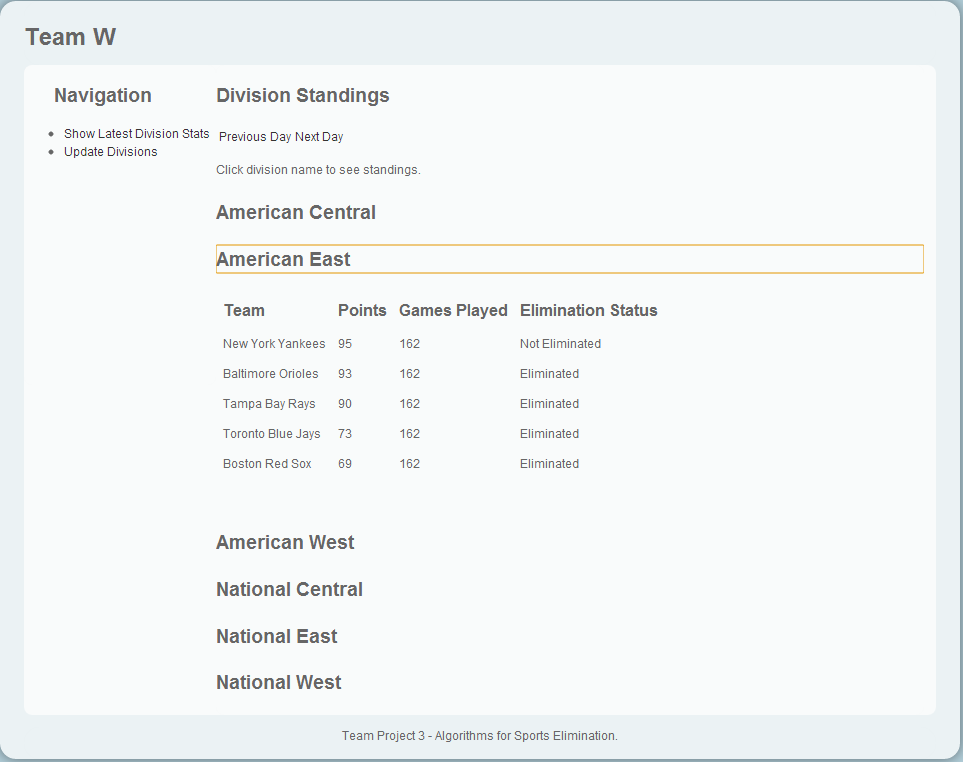
\includegraphics[width=\linewidth,keepaspectratio]{images/userManualWeb2.png}
\caption{Web Application Details}\label{fig:WEBINFO}
\end{figure}

To navigate between different days you can use the previous/next day buttons
above the leagues and divisions or by direct URL manipulation as shown
in Figure~\ref{fig:WEBNAV}. Finally, if you'd like to jump back to the
latest results in a given season click ``Show Latest Division Stats''
in the side navigation bar.

\begin{figure}
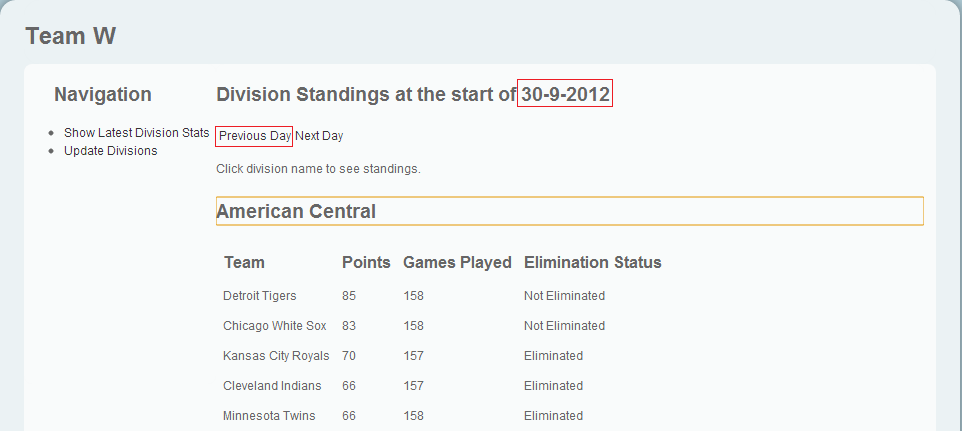
\includegraphics[width=\linewidth,keepaspectratio]{images/userManualWeb3.png}

\includegraphics[width=\linewidth,keepaspectratio]{images/userManualWeb4.png}
\caption{Web Application Navigation}\label{fig:WEBNAV}
\end{figure}

